\documentclass[5p,times]{sig-alternate-05-2015}

\usepackage{etoolbox}
\makeatletter
\patchcmd{\maketitle}{\@copyrightspace}{}{}{}
\makeatother

\begin{document}

\doi{}

\title{Student Cluster Competition 2018, Team Tsinghua University: Reproducing the SeisSol Optimization on Intel Skylake Architecture}
\newcommand\OriginalPaper{the Sumatra paper}

\numberofauthors{1}
\author{
\alignauthor
Chenggang Zhao\textsuperscript{*}, Jia'ao He\textsuperscript{*}, Jiping Yu, Chenyao Lou, Xinjian Yu and Liyan Zheng\\
\vspace{5pt}
       \affaddr{Department of Computer Science and Technology}\\
       \affaddr{Tsinghua University, Beijing, China}\\
\vspace{5pt}
       \email{\textsuperscript{*}~zhaocg17@mails.tsinghua.edu.cn, hja16@mails.tsinghua.edu.cn}\\
}

\maketitle

% ----------------------------------------------------- %
\begin{abstract}

% REQ: Write two or three sentences describing this manuscript. Include goals of the report and a brief description of the platform on which the work is done. %
A paper entitled ``\textit{Extreme Scale Multi-Physics Simulations of the Tsunamigenic 2004 Sumatra Megathrust Earthquake}'' in SC'17 implemented a new cache-aware wave propagation scheme and an optimization approach for dynamic rupture using code generation. With the clustered local time-stepping method, they archived a 13.6$\times$ speedup for the Sumatra scenario of the simulation code SeisSol.

In this work, we reproduce the optimization approach above on Intel Skylake, a relatively new architecture, to analyze its performance. We compare the performance results obtained on our platform with those in the original paper and study the differences with a profiling-based performance tool, Arm Forge. We perform scalability experiments on our cluster with the provided dataset. In particular, a full $500$-second simulation of the Sumatra earthquake on a small mesh is successfully reproduced on our platform.

Results show that an apparent performance gain is obtained on our platform, which is consistent with the claims in the original paper. Furthermore, we also analyze the impact of hyper-threading on the performance.

\end{abstract}

\keywords{Reproducibility; Cache; Scalability; Earthquake simulation; Student Cluster Competition.}

% ----------------------------------------------------- %
% REQ: Give a description of the SeisSol paper, and the claims from the paper you are trying to reproduce. %
\section{Introduction}

The $M_w$ 9.1 Sumatra-Andaman Earthquake was a megathrust earthquake, which killed around 280,000 people and triggered a series of large tsunamis up to 30 metres high. Though there is a long way to go for accurate earthquake prediction, effective simulations for earthquake can help people better understand the earthquake itself.

Uphoff, Rettenberger, Bader, et al. archived a 500s-1500km multi-physics simulation for the Sumatra scenario in their SC'17 paper titled ``\textit{Extreme Scale Multi-Physics Simulations of the Tsunamigenic 2004 Sumatra Megathrust Earthquake}''~\cite{Uphoff:2017:ESM:3126908.3126948}, which we will refer to as ``\OriginalPaper'' in our report. To resolve such large-scale frictional sliding and wave propagating processes, they have proposed several end-to-end optimization techniques in their paper, including:

\begin{description}

\item [Better cache utilization] Flux matrix decomposition and KNL L2 cache prefetching.

\item [Code generation] Using libxsmm library and auto-tuning for small-size matrix multiplications.

\item [Asynchronous output] I/O thread and direct I/O are supported.

\item [LTS] Using local time-stepping method~\cite{LTS:7516082}.

\end{description}

With these optimization techniques listed above, on the Sumatra scenario dataset, the time-to-solution was reduced to 13.9 hours on 86,016 Haswell cores of SuperMUC, achieving a 13.6$\times$ speed-up over the baseline.

In this report, we reproduce the proposed approaches in \OriginalPaper{}, including \textbf{the single node performance on the proxy} and \textbf{scalability from the view of sockets}. Also, we perform the \textbf{visualization output experiment} to verify the results of a full $500$-second simulation of the Sumatra earthquake.

% ----------------------------------------------------- %
% REQ: Describe the details of your cluster include whatever is relevant for your report %
\section{Reproduction Environment}
\subsection{Hardware Configuration}
Our cluster that is used to reproduce the results of \OriginalPaper\ is set up as listed in Table~\ref{tab:hw}.

\begin{table}[h]
\centering

\begin{tabular}{|l|l|}
\hline
Nodes & \begin{tabular}{@{}c@{}}Supermicro SuperServer \\4029GP-TRT2 $\times$ 2 \\7049GP-TRT $\times$ 2 \end{tabular} \\ \hline
CPU per node & Intel Xeon Platinum 8176 $\times$ 2 \\ \hline
Memory per node & DDR4 2666 MT/s 16 GB $\times$ 12 \\ \hline
Storage on the head node & \begin{tabular}{@{}c@{}}Intel SSD DC P3608 4TB + \\ Intel SSD DC S4600 960GB \end{tabular}   \\ \hline
Storage on other nodes & Intel SSD DC S3610 100GB \\ \hline
Infiniband per node & Mellanox EDR adapter \\ \hline % 删去了x2
Ethernet per node & 10GBase-T LAN adapter \\ \hline
Operating System & Debian 9.5 \\ \hline
Kernel & Linux kernel 4.9.110 \\
\hline
\end{tabular}
\caption{Environment Specification}
\label{tab:hw}
\end{table}

Each node is equipped with 2 \textit{Intel Xeon Platinum 8176}, which has 28 cores per socket in support of AVX-512, 32KB L1d/i cache, 1MB L2 cache per core and a 38.5MB shared L3 cache at a AVX-512 based frequency of 1.3 GHz. With these processors, we can use vectorized instructions up to 512 bits wide and get a much higher performance benefited from a larger cache, a 126 GB/s memory bandwidth of hexa-channel, and hyper-threading technology. Furthermore, the differences in architecture between our platform and the original platform, such as cache size and vector length, have large impact on the performance, and we will elaborate these points in this work. 

\subsection{Software Environment}

The compilers, libraries, and running environment are listed in Table~\ref{tab:sw}.

\begin{table}[ht]
\centering

\begin{tabular}{|l|l|}
\hline
Compilers & Intel C++ and Fortran Compilers 2017 \\ \hline
MPI & Intel MPI Library 2017 \\ \hline
libxsmm & 1.9 \\ \hline
HDF5 & 1.8.11 \\ \hline
netCDF & 4.3.0 \\ \hline
\end{tabular}
\caption{Compilers, libraries, and environment}
\label{tab:sw}
\end{table}

% 这里说的是为啥用Intel 2017而不是2018 %
The reason why we choose Intel Compiler 2017 instead of 2018 or 2019 is that the directive ``\#pragma simd'' used in the SeisSol code is removed from the version of 2018. And changing the code may affect the behavior of SeisSol.


For libxsmm, HDF5, and netCDF, the versions mentioned in the GitHub wiki\footnote{https://github.com/SeisSol/SeisSol/wiki/Compilation} are used.

% ----------------------------------------------------- %
\section{Compilation and Run}
\subsection{Code Versions}
To get more convincing results, we use the Shaking Corals\footnote{https://github.com/SeisSol/SeisSol/tree/201703} and Baseline\footnote{https://github.com/SeisSol/SeisSol/tree/sc17\_baseline} versions of SeisSol in \OriginalPaper{}'s artifact description, following the instructions given by the authors.

For single node performance which is measured by a proxy program mentioned in \OriginalPaper, we use the version provided by the authors, which was a previous commit to the ``libxsmm'' repository\footnote{https://github.com/hfp/libxsmm \\ Commit ID: b62a68824bd8fe2c48bf0139264a088021df5e64}.

% REQS:
% Describe the steps to compile/run the software for your machine.
% Include command line parameter and scripts you used.
% Include which ​small matrix multiplication kernels (SMMs) you used and the location pulled from. Describe the necessary steps of modification and optimization for your hardware architecture.%

\subsection{Compilation}
% AVX-512 %

As we have ``AVX-512'' vectorization support on our platform, guided by the authors, we add the new ``skx'' architecture in the project. We follow the instructions from GitHub wiki\footnote{https://github.com/SeisSol/SeisSol/wiki/Optimization-for-non-Intel-architectures}. Specifically, we change the architecture option to ``skx'' (AVX-512 option for Intel Xeon processors, which libxsmm also supports), modify the compilation flags with ``-xCORE-AVX512'', and set the alignment length to 64.

After getting the tuned memory layouts which will be discussed in the following sections, we compile both the proxy and the main program. The libxsmm code generator is used to generate the matrix multiplication kernels. We run the ``scons'' to build the main program as described in the wiki. Following the wiki, we use the compilation flag ``commThread'' for better communication. Also, the support of AVX-512 Skylake architecture is enabled with a flag of ``dskx''.

\subsection{Auto Tuning}
For better performance of matrix multiplication, auto-tuning for matrix memory layout is used in \OriginalPaper\ along with libxsmm code generation. For the Shaking Corals version, we run the script ``auto\_tune.py'' in the SeisSol auto-tuning directory with parameters of ``nelem=100000'' and  ``ntimesteps=500'' to get better performance on Skylake processors. Finally, we archive a speed-up of approximately 20\% in the case of order 7. 

The baseline version is also tuned using its auto tuning script, which is provided in the ``seissol\_kernel'' subrepository. The script is serial, and the code generation process is completed by a serial Python script. To accelerate the code generation, we improve the script's workflow, and parallelize the code generation for better efficiency.

% ----------------------------------------------------- %
\section{Reproduction Work}

The reproduction work in 2018 student cluster competition consists of three parts listed below. 

\begin{description}
\item [Single node performance] The single node performance of the wave propagation, tested on a proxy program. Also the impact of hyper-threading and the details of hardware counters need to be reported.

\item [Scalability from the view of sockets] The experiment is conducted on our 4-node cluster, studying the scalability from the view of sockets.

\item [Visualization verification] We try to reproduce the same model of the Sumatra megathrust earthquake but on a much smaller mesh, to compare with the output in the original paper and analyze the differences.
\end{description}

% +++++++++++++++++++++++++++++++++++++++++++++++++++++ %
\subsection{Single Node Performance}

In \OriginalPaper, a better use for the flux matrices of cache was achieved by doing matrix decomposition, code generation, and auto-tuning. In Figure 2 and 3 of \OriginalPaper, a significant improvement was claimed in the case that the size of flux matrices is larger than the L2 cache. The experiments were conducted on a proxy with random data, compared with the baseline (BL) version and Shaking Corals (SC) version.

Due to the lack of Knight Landing processors, we cannot reproduce the results with prefetching. We only measure the performances of BL and SC version with different orders on Skylake processors. The results are shown in Figure~\ref{fig:single}.

% NOTE: 这里是neighbor flux kernel的加速比的图 %
\begin{figure}[!ht]
	\centering
	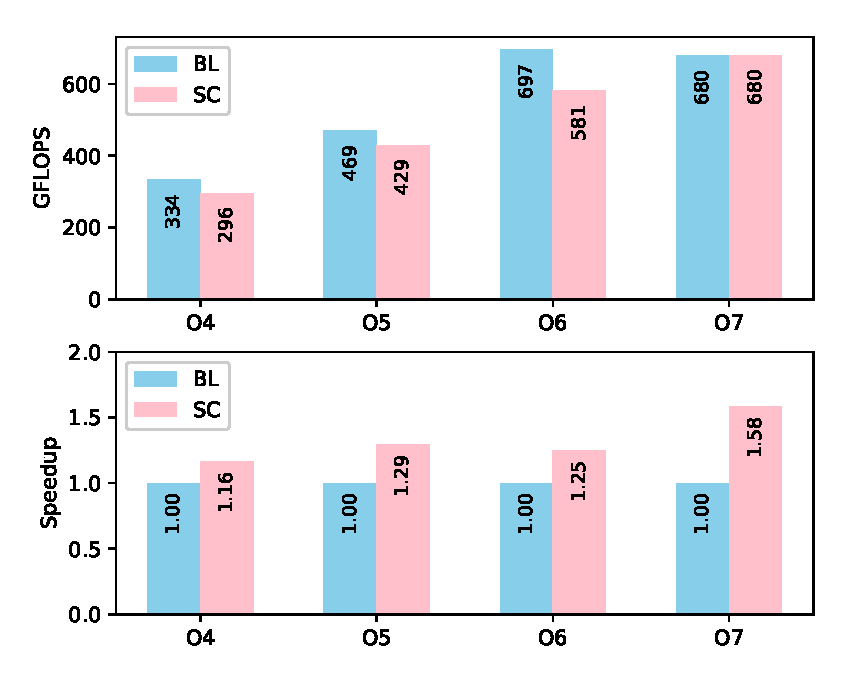
\includegraphics[width=0.45\textwidth]{singlenode.eps}
	\caption{GFLOPS and speedup of the wave propagation caused by matrix decomposition, code generation, and auto-tuning. This experiment is carried out on the proxy with 100,000 elements and 1,000 timesteps from the orders O4 to O7. Figures show a high consistency with the \OriginalPaper.}
	\label{fig:single}
\end{figure}

Figure~\ref{fig:single} shows the speedup of the wave propagation for the BL and SC versions. As the size of the flux matrices of BL is getting larger towards exceeding our L2 cache size, the superiority of the SC version is much more obvious. The main reason is that there is a much higher possibility for the matrices to reside in L3 cache, which was also claimed in \OriginalPaper. From the perspective of machine usage, SC achieves up to 29\% of the peak performance on our Skylake processors (AVX-512 based frequency of 1.3 GHz) in the case of order 7, while BL achieves 29\%.
% 上面这两个数我不100%保证算对? 0.29 = 680 / (1.3 * 28 * 32 * 2) % 
% Node performance in GFlops = (CPU speed in GHz) x (number of CPU cores) x (CPU instruction per cycle) x (number of CPUs per node)

For a deep analysis, we use Arm Forge profiler to record hardware counters to get the overview of a single run. As a result, in the case of order 7, the BL version spends 85.9\% of the time on memory access with total L2 misses of 3,698 million instructions (only the main thread is measured due to the limitation of the profiler), while the SC version only spends 56.5\% of time on memory access with total L2 misses of 840 million instructions (only the main thread). Figure~\ref{fig:arm} is a screenshot of the Arm Forge profiler showing the important performance figures of the run.

% NOTE: 这里是一个运行截图 %
\begin{figure}[!ht]
	\centering
	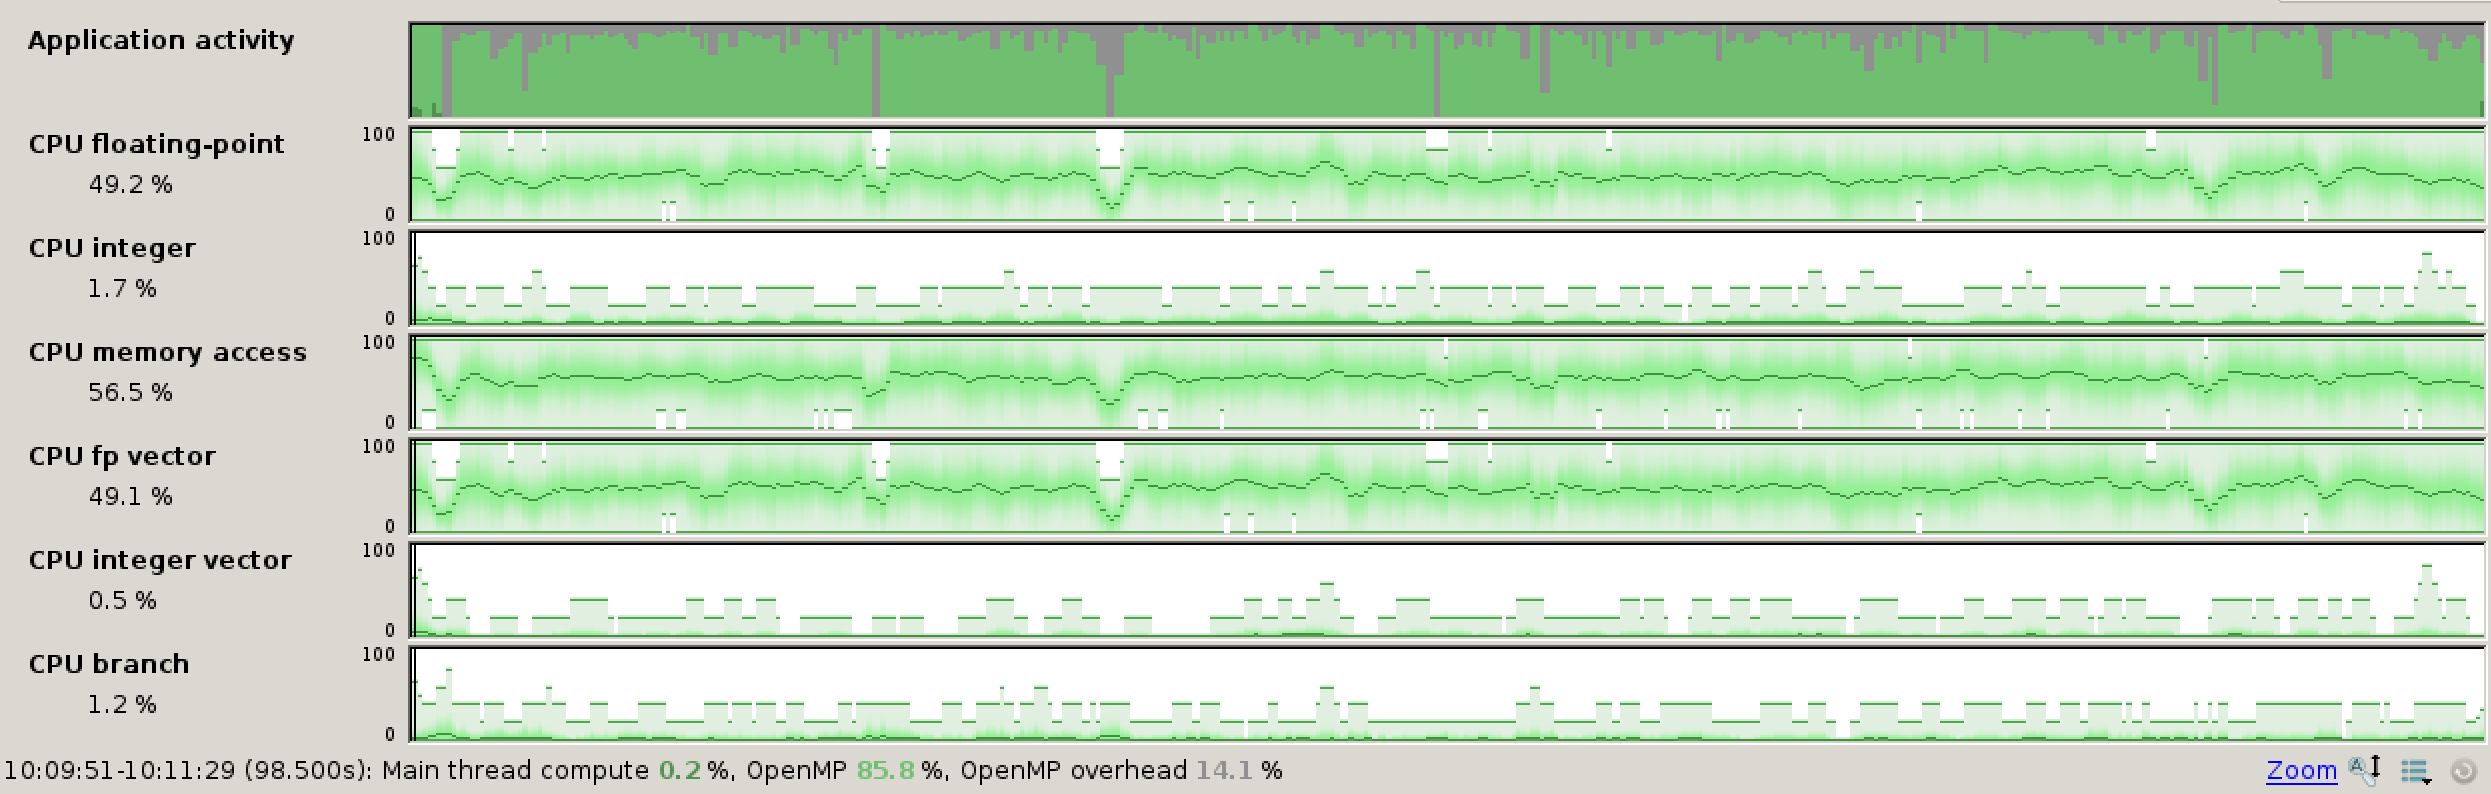
\includegraphics[width=0.45\textwidth]{arm.png}
	\caption{A screenshot of the Arm Forge profiler shows an overview of a run of the SC version, which can help diagnose the performance quickly and efficiently.}
	\label{fig:arm}
\end{figure}

An interesting fact we discover in our experiments is that the impact of hyper-threading to the memory-accessing-sensitive Baseline is very large, especially for the order of 7. All the results in our experiments are reproduced with hyper-threading on, but by coincidence we find that a performance improvement of 20\% on the BL version is achieved in the case of 7 without hyper-threading. We use Arm Forge to analyze this behavior. The results of Arm Forge show us a drop of L3 cache performance due to the cache contention of more logical threads with hyper-threading on. However, in the cases of other orders and the SC version, flux matrices are not large enough to trigger such problem so they can benefit from hyper-threading. 

% +++++++++++++++++++++++++++++++++++++++++++++++++++++ %
\subsection{Scalability from the View of Sockets}

\subsubsection{GTS and LTS Algorithms}
In earthquake simulations in realistic scenarios, the scalability is even more important, as the scale of the dataset is much larger. In this Section, we reproduce the results in \OriginalPaper\ and analyze the differences between the global time-stepping method (GTS) and local time-stepping method (LTS) on our platform. The maximum length of timestep for a certain element depends on the Courant-Friedrichs-Lewy (CFL) condition, which varies between elements. In GTS, the minimum time step of all elements is applied as the length of time step for all elements, causing a waste of computing resources. The aim of LTS is to increase the length of time step of some elements. To solve the problem of flux passing between elements that share a face with different time step, high level deviations are calculated for the elements with a larger time step, in order to calculate the flux matrix of the elements with a smaller time step by using the formulation of the ADER time integration~\cite{LTS:7516082}. 

For the convenience of programming, the size of time steps is usually set to some specific value in a geometric series. The common ratio of the series is usually $2$ or $3$. If it is set to $1$, the algorithm becomes GTS.

\subsubsection{Scalability Experiments}

As our cluster only has 4 computing nodes and 8 CPU processors in total, we perform scalability experiments with up to 8 CPU processors.

%Due to lack of nodes, here we do a strong scaling study by the number of sockets (28 physical CPU cores per socket).

The real 2004 Sumatra dataset provided during the competition is used, but on a relatively small mesh. In the scalability experiment, we estimate the full execution time by setting the simulation time to $2s$. To get more data points, we use different numbers of CPU processors to analyze the scalability in Figure~\ref{fig:sca}.


The environment variable of ``OMP\_NUM\_THREADS'' is set to ``56'' for consistency, and ``KMP\_AFFINITY'' is set to ``compact,granularity=thread'' as mentioned in~\OriginalPaper\ to bind the program to a specific socket.

% NOTE: 这里是Scalability实验的图 %
\begin{figure}[!ht]
	\centering
	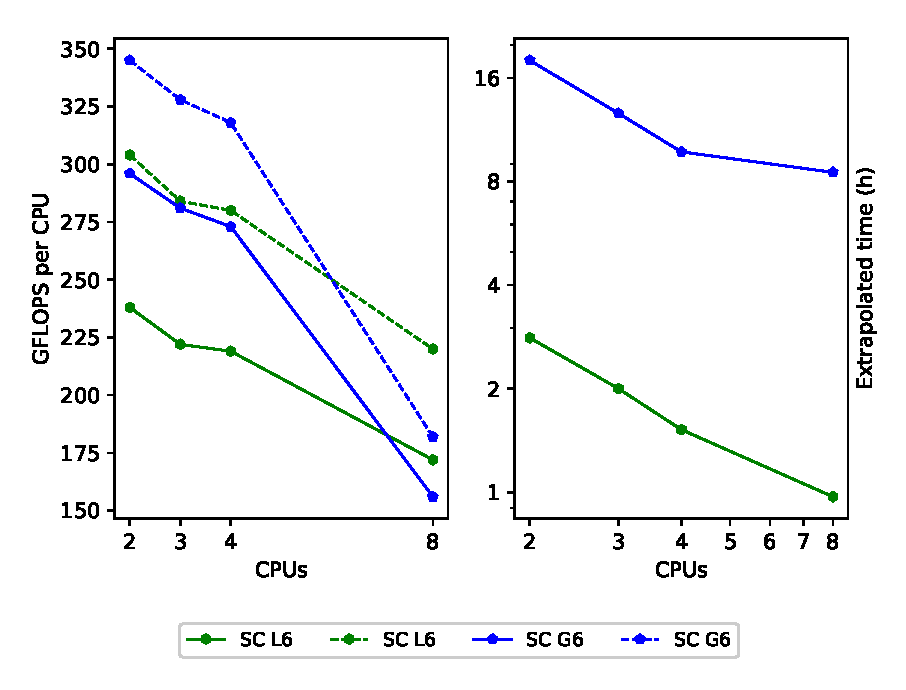
\includegraphics[width=0.45\textwidth]{scale.eps}
	\caption{The scalability of the two versions on our cluster by different numbers of CPU processors. The left part shows a performance of GFLOPS, while the right part is an extrapolated time of the full 500-second simulation.}
	\label{fig:sca}
\end{figure}

% HJA %
From the figure, we can see that a good scalability is achieved when the number of CPU processors is no more than 4. However, the performance drops greatly when it comes to the experiment with $8$ CPU processors on $4$ computing nodes. This is because that, to save the power in our competition, we do not use Infiniband switch in our cluster. We only have Infiniband network connection between two nodes. Ethernet connection is used otherwise. Therefore, the mixed network configuration of our cluster causes the drop of performance. 

%The mixed configuration of our cluster is reasonable for this phenomenon. We only have $2$ out of all the $4$ nodes interconnected to each other by InfiniBand. The Ethernet which is only designed to be used as control network was very unstable during the competition, making communication the bound of the program.

The computational behavior is consistent throughout the whole process. Therefore, the first several iterations can represent the following computation. Therefore, we decide to use the first $2$ seconds from the $500$ seconds to represent the whole period of experiments, and use $250$ times of its duration as our estimation to the final running time.


\subsubsection{Load Balance}
In our version of SeisSol, meshes are pre-divided in the mesh file into different partitions, which will be run in different threads. We compile ``PUML'' repository \footnote{https://github.com/TUM-I5/PUML} with Metis\footnote{https://github.com/scibuilder/metis}. 

Metis is used to automatically divide the graph in which elements are regarded as vertices, and faces are regarded as edges, into the required partitions for parallelism. As mentioned in~\cite{LTS:7516082}, the weight of a vertices $w_l$ is set to $\Pi_{i=l-1}^L r_i$, which means the number of iterations it needs to compute during one iteration of the element with the longest time, which is an approximate estimation of the load that the element has. By equally partitioning the elements into different partitions, the computation load can be evenly distributed.

Results are shown in Figure~\ref{fig:lb}, which is based on the number of elements in each time step generated by the main program of SeisSol. The figure demonstrates the even distribution of rupture faces and elements. It also suggests that local time stepping saves a lot of computational resources by reducing the total amount of calculation required.

% NOTE: 这里是Load Balance实验的图 %
\begin{figure}[!ht]
	\centering
	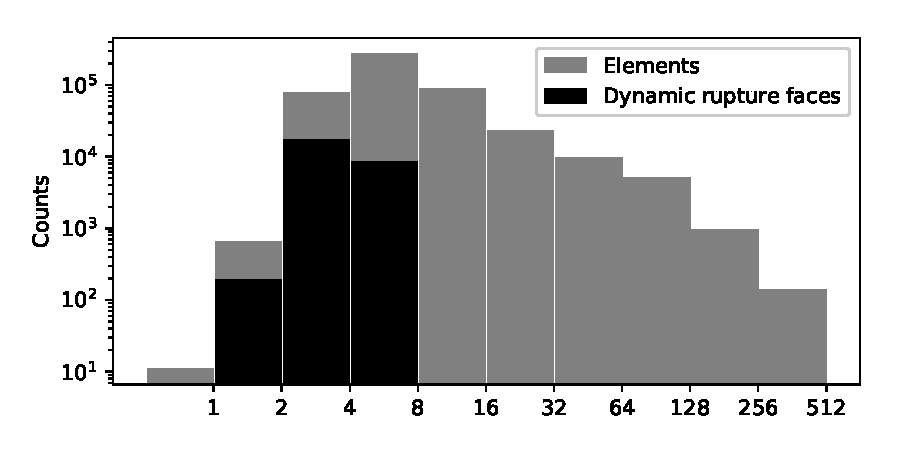
\includegraphics[width=0.45\textwidth]{load.eps}
	\caption{Distribution of elements and dynamic rupture faces to time clusters. The sockets which cover the range $[4\Delta t_{min}, 64\Delta t_{min})$ contain 96.7\% of elements.}
	\label{fig:lb}
\end{figure}

% +++++++++++++++++++++++++++++++++++++++++++++++++++++ %
\subsection{Visualization Verification}
It is required to run $500$-second simulation on the same dataset to observe the process of the earthquake. The result is conducted smoothly with $CFL=0.5$ in the case of order 4.

After the run is done, we use ParaView to analyze the result of the surface. We calculate the horizontal displacement by $d_h=\sqrt{U^2+V^2}$ and vertical displacement by $d_v=W$, where $U$, $V$ and $W$ are the results from the output.

\begin{figure}[!ht]
	\centering
	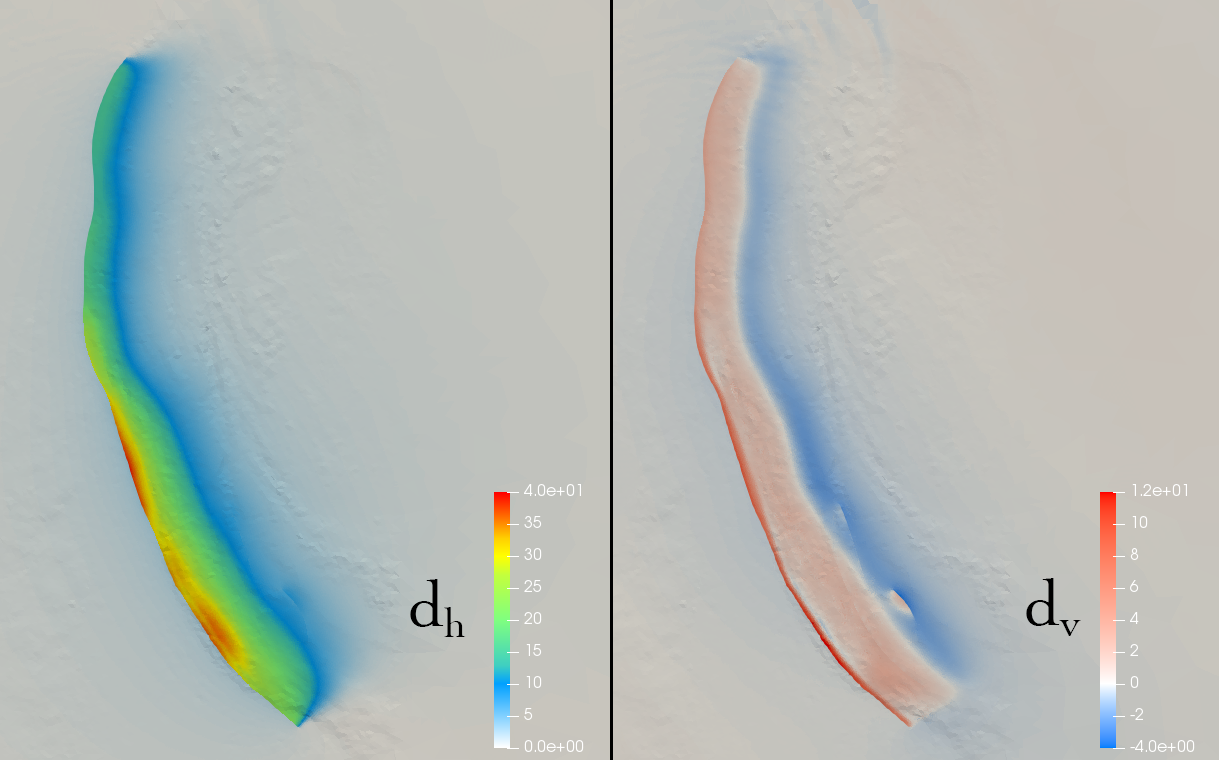
\includegraphics[width=0.45\textwidth]{geo.png}
	\caption{Horizontal (left) and vertical (right) movement of the elements on the seafloor after 500-second simulation.}
	\label{fig:geo}
\end{figure}

In Figure~\ref{fig:geo}, horizontal and vertical seismic waves propagate from one point and spread all around in the area in several tens of seconds. And it is highly consistent with Figure~9 in \OriginalPaper, which verifies our modification for Skylake processors.

% ----------------------------------------------------- %
\section{Conclusions}

In this work, we reproduce both \textbf{Single node performance} and \textbf{Scalability} experiments in \OriginalPaper. We also do the verification by comparing \textbf{Visualization Outputs}. Results on our platform show that the three major experiments are consistent with the conclusions made in \OriginalPaper. 

In our experiments, we find that Intel Skylake processors have much better performance than previous processors. The program that we optimize on our new processors obtains certain speedup over the original version.

%without changing the properties of traditional architecture like cache.

As asynchronous MPI point-to-point communications are used in this program and a limited number of faces can be attached to a certain element, we find that this program is not very communication-bounded. We get a good scalability on our platform.

The result of our simulation for the wave propagation animation can be used potentially for geologists to analyze the earthquake. The successful compilations and optimization for this program make us finish all the simulations within 48 hours.

% ----------------------------------------------------- %
\bibliographystyle{abbrv}
\bibliography{sigproc.bib}

\end{document}
